\documentclass{beamer}
\usepackage[utf8]{inputenc}
\usepackage{textcomp}
\usepackage{tipa}
\usepackage{appendixnumberbeamer}

\usepackage{graphicx}
\graphicspath{{images/}}
\usepackage{colortbl}

%\usepackage{parskip}
\setlength{\parskip}{\baselineskip}

\usepackage{fontspec}
\newfontfamily\ipafamily{DejaVu Sans}[Scale=MatchLowercase]
\DeclareRobustCommand\ipa[1]{{\ipafamily/#1/}}

\usetheme[hideothersubsections]{Berkeley}
\usecolortheme{crane}
\usefonttheme{structuresmallcapsserif}
\setbeamertemplate{navigation symbols}{}
\usefonttheme[onlymath]{serif}
\setbeamertemplate{bibliography item}{}

\newcommand{\realtilde}{\char`\~}

\title{How fast did Cicero speak?} \subtitle{The speech rate of Classical Latin versus its Romance descendants}
\author{Daniel Stelzer}
\institute{University of Illinois at Urbana-Champaign}
\date{Stage 1 Qualifying Exam}

\begin{document}

\frame{\titlepage}

\section{Background}

\subsection{Speech Rate}

\begin{frame}{Speech Rate}
It's widely known that languages are spoken at different rates

This can be measured quantitatively: time speakers reading a prepared text, remove pauses, divide by the number of syllables in the text

This ``speech rate'' (syllables per second) varies significantly between languages: despite individual variation, Spanish and Italian are generally spoken faster than English and Hungarian
\end{frame}

\subsection{Info Density}

\begin{frame}{Information Density}
It's also widely known that languages have different syllable inventories

Maximal syllables:
\vspace{-1em}
\begin{itemize}
    \item Japanese: CjVn (\ipa{kjuɴ} ``overcome with emotion'')
    \item English: sCCVCCC (\ipa{stɹɛŋθs} ``strengths'')
    \item Georgian: unlimited? (\ipa{gvprtskvnis} ``he is peeling us'')
\end{itemize}

\emph{We focus specifically on languages where ``syllables'' make sense as a meaningful unit---moreso in English than in Georgian}
\end{frame}

\begin{frame}{Information Theory}
How much actual information does each syllable convey?

If we know with 100\% certainty what the next syllable will be, hearing it gives us no new information at all

But if it could be any of a hundred different options, it conveys much more information (namely, which of those hundred it is)

And if it could be any of a \emph{thousand}, that conveys even more information

Information theory lets us measure this quantitatively: the entropy or ``information density'' in bits per syllable
\end{frame}

\subsection{Info Rate}

\begin{frame}{Information Rate}

Multiplying these two values gives the ``information rate'' in bits per second

Coupé et al 2019: this value is more consistent between languages than either speech rate or information density!

In other words, different languages convey approximately the same amount of information per second---if there's more information per syllable, there are fewer syllables per second, and vice versa
\end{frame}

\begin{frame}{Information Rate}
This may be a fundamental property of the human ``communicative niche'', the way we communicate as a species

We can't measure the speech rate of dead languages, since there are no native speakers

But we \emph{can} calculate the information density if we have large enough written corpora

\textbf{Can we reverse-engineer the speech rate from that?}
\end{frame}

\section{Methods}

\subsection{Entropy}

\begin{frame}{}
\begin{center}
\textbf{\Large Step 1: Calculating Information Density}
\end{center}
\end{frame}

\begin{frame}{Shannon Entropy}
The classical formulation of entropy: how much information do we get from a syllable, on average?

\[H = - \sum_{\textrm{syllable}} P(\textrm{syllable}) \log P(\textrm{syllable})\]

Rationale: this definition captures both how many possibilities there are, and how likely they are to appear

But it only looks at syllables in isolation
\end{frame}

\begin{frame}{Conditional Entropy}
``Conditional entropy'': how much information do we get from a syllable, on average, when we already know the context?

\[ID = - \sum_{\substack{\textrm{syllable},\\\textrm{context}}} P(\textrm{context}, \textrm{syllable}) \log \frac{P(\textrm{context}, \textrm{syllable})}{P(\textrm{context})}\]

In this case, the ``context'' is the preceding syllable within the same word

Oh 2015: this is a good measure of information density

How much the context matters varies by language
\end{frame}

\subsection{Representation}

\begin{frame}{}
\begin{center}
\textbf{\Large Step 2: Identifying Syllables}
\end{center}
\end{frame}

\begin{frame}{Orthography}
Latin orthography is remarkably consistent, thanks to scribal transmission

But not quite phonemic:
\vspace{-1em}
\begin{itemize}
    \item \textsc{alivm} \ipa{a.li.um} ``another''
    \item \textsc{alivm} \ipa{aː.li.um} ``garlic''
    \item \textsc{volvit} \ipa{wo.lu.it} ``she wanted''
    \item \textsc{volvit} \ipa{wol.wit} ``it rolls''
    \item \textsc{ivlvs} \ipa{i.u.lus} ``Iulus (name)''
    \item \textsc{ivlivs} \ipa{ju.li.us} ``Julius (name)''
\end{itemize}

``Augmented'' or ``annotated'' orthography:\\
\quad\emph{\textbf{a}lium} vs \emph{\textbf{ā}lium}, \emph{vol\textbf{u}it} vs \emph{vol\textbf{v}it}, \emph{\textbf{I}ulus} vs \emph{\textbf{J}ulius}

Winge 2015: automatic annotation, over 98\% accuracy
\end{frame}

\begin{frame}{Phonemic Representation}
Converting augmented orthography to phonemic representation is straightforward; very few changes needed
\vspace{-1em}
\begin{itemize}
    \item \emph{exit} → \emph{ecsit} ``he leaves''
    \item \emph{Karthāgō} → \emph{Carthāgō} ``Carthage (city)''
    \item \emph{quīnque} → \emph{\(\varkappa\)īn\(\varkappa\)e} ``five''
\end{itemize}

\textbf{Most phonetic details are ignored}

First exception: where it impacts syllabification
\vspace{-1em}
\begin{itemize}
    \item \emph{majus} → \emph{majjus} ``greater''
\end{itemize}
\vspace{-0.75em}
Second exception: complete neutralization
\vspace{-1em}
\begin{itemize}
    \item \emph{equus} → \emph{ecus} ``horse''
    \item \emph{urbs} → \emph{urps} ``city''
\end{itemize}
\end{frame}

\begin{frame}{Syllabification}
Fortunately, syllabification is mostly a solved problem

Classical-era poetry treated closed and open syllables differently

So scholars have been formalizing syllabification rules since the Renaissance (if not earlier) based on Virgil and Ovid

(Sanity check: coda consonants also affected stress, which caused sound changes in Romance)

Algorithm from CLTK, with some enhancements: boils down to ``maximize onsets''
\end{frame}

\subsection{Extrapolation}

\begin{frame}{}
\begin{center}
\textbf{\Large Step 3: Extrapolation}
\end{center}
\end{frame}

\begin{frame}{Corpora}
Entropy can be estimated from a sufficiently large corpus

English Wikipedia:\\\quad\realtilde{}4,000,000,000 tokens (4 billion)

The entire surviving corpus of Classical Latin literature:\\\quad\realtilde{}7,000,000 tokens (7 million)

Is this ``sufficiently large''?
\end{frame}

\begin{frame}{Bootstrapping}
Bootstrapping is a classic way of artificially enlarging a dataset

But with natural language, Zipf's Law (and Heaps' Law) means that many perfectly-valid words only appear once in the corpus---and even more never appear at all

\emph{Audīverās} ``you had heard'' appears only once (Terence's \emph{Phormio}, line 573)

\emph{Audīverint} ``they might have heard'' is unattested, completely by accident

Bootstrapping will very often turn a frequency of 1 to 0, but will never turn a frequency of 0 to 1
\end{frame}

\begin{frame}{Extrapolation}
\emph{Reducing} the dataset works well: discard tokens at random until you reach the desired size

Can we use this to extrapolate out to an infinitely-large corpus?
\end{frame}

\begin{frame}{Extrapolation}
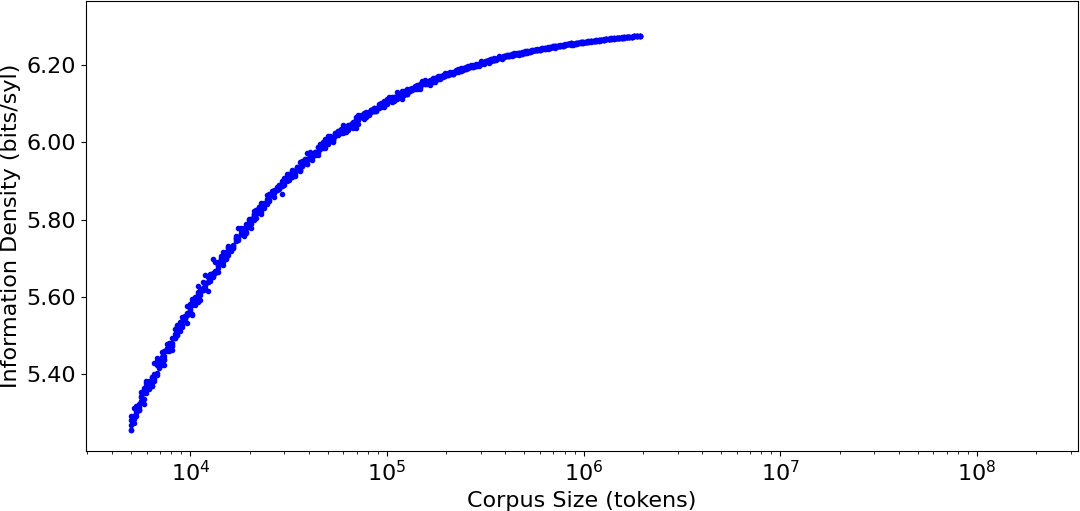
\includegraphics[width=\linewidth]{demo1}
\vspace{-2ex}
\[\quad\]
\end{frame}

\begin{frame}{Extrapolation}
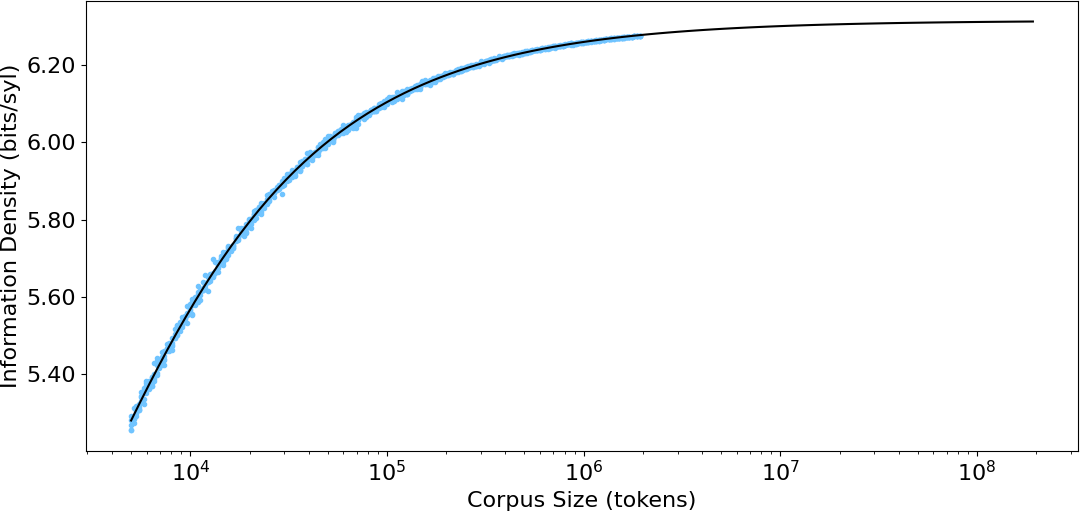
\includegraphics[width=\linewidth]{demo2}
\vspace{-2ex}
\[y=a-b(x-c)^{-d}\]
\end{frame}

\begin{frame}{Extrapolation}
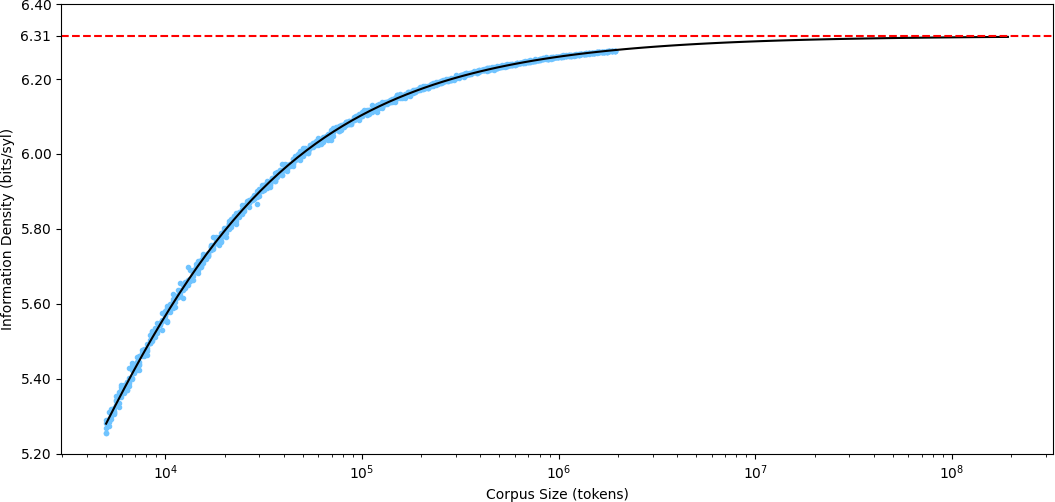
\includegraphics[width=\linewidth]{demo3}
\vspace{-2ex}
\[y_{\infty}=a\]
\end{frame}

\subsection{Jackknifing}

\begin{frame}{}
\begin{center}
\textbf{\Large Step 4: Uncertainty}
\end{center}
\end{frame}

\begin{frame}{Limitations}
Theoretically, we can use this extrapolation on any corpus, no matter how small

But the smaller the corpus, the less information we have---how do we know that what survived is representative of the language as a whole?

Assumption: differences between authors are greater than differences between works

In other words, Gallus would have more of an impact than Ovid's \emph{Medea}
\end{frame}

\begin{frame}{Jackknifing}
We can't know how many authors are lost, or how much they would have differed from what survived

But we can calculate how much impact each surviving author has on our results, by \emph{removing} them one at a time

The variance in these results gives an estimate of how much a missing author could affect things
\end{frame}

\section{Results}

\subsection{Corpus}

\begin{frame}{Corpus Selection}
The Packard Latin Corpus: ``essentially all Latin literary texts'' from before 200 CE, plus a few prominent later works

Prose, poetry, fragments, quotations…anything that's recognizably Latin and part of a published work (so no graffiti or inscriptions)

Authors with >100,000 tokens used for jackknifing
\end{frame}

\begin{frame}{Corpus}
\begin{table}
\begin{tabular}{|c|c|c|c|c|}
\hline
\textbf{Author} & \textbf{Genre} & \textbf{Century} & \textbf{Types} & \textbf{Tokens} \\\hline
\textbf{Total} & & & 329,228 & 7,240,473 \\\hline\hline
Cicero & Everything & 1st BCE & 85,020 & 1,165,502 \\\hline
Justinian & Law & 6th CE & 40,599 & 852,973 \\\hline
Livy & History & 1st BCE & 55,308 & 520,674 \\\hline
Pliny & Science & 1st CE & 68,237 & 392,178 \\\hline
Servius & Grammar & 4th CE & 52,524 & 373,819 \\\hline
Seneca & Philosophy & 1st CE & 50,723 & 362,937 \\\hline
Quintilian & Rhetoric & 1st CE & 40,092 & 321,209 \\\hline
Ovid & Poetry & 1st BCE & 36,787 & 222,745 \\\hline
\end{tabular}
\end{table}
\end{frame}

% NOTE - this is a copy of the previous frame with the top two rows colored in, so make sure you edit both
\begin{frame}{Corpus}
\begin{table}
\begin{tabular}{|c|c|c|c|c|}
\hline
\textbf{Author} & \textbf{Genre} & \textbf{Century} & \textbf{Types} & \textbf{Tokens} \\\hline
\textbf{Total} & & & 329,228 & 7,240,473 \\\hline\hline
\rowcolor{yellow} Cicero & Everything & 1st BCE & 85,020 & 1,165,502 \\\hline
\rowcolor{yellow} Justinian & Law & 6th CE & 40,599 & 852,973 \\\hline
Livy & History & 1st BCE & 55,308 & 520,674 \\\hline
Pliny & Science & 1st CE & 68,237 & 392,178 \\\hline
Servius & Grammar & 4th CE & 52,524 & 373,819 \\\hline
Seneca & Philosophy & 1st CE & 50,723 & 362,937 \\\hline
Quintilian & Rhetoric & 1st CE & 40,092 & 321,209 \\\hline
Ovid & Poetry & 1st BCE & 36,787 & 222,745 \\\hline
\end{tabular}
\end{table}
\end{frame}

\begin{frame}{The Digesta}
The PHI corpus includes ``some texts selected from later antiquity''

The most prominent is the \emph{Digesta} of Emperor Justinian: a sixth-century attempt to compile all legal precedents from all of history

50 volumes, relatively formulaic and repetitive text
\end{frame}

\begin{frame}{The Digesta}
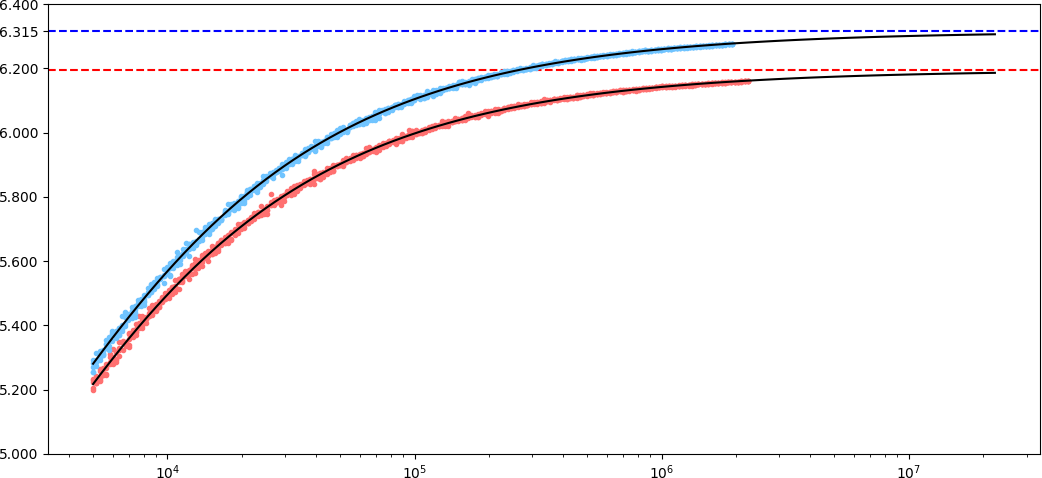
\includegraphics[width=\linewidth]{digesta}
\end{frame}

\begin{frame}{Cicero}
Cicero was absurdly prolific---approximately 75\% of the surviving writing from his time period is his

Looking at the entire corpus, \realtilde{}20\% of it is Cicero (1,165,502 tokens out of 6,387,500)

Unlike the \emph{Digesta}, this is definitely Classical Latin, and should be included in the calculations

But what about jackknifing?
\end{frame}

\subsection{Entropy}

\begin{frame}{Entire corpus}
\includegraphics[width=\linewidth]{latin}

ID = 6.216 bits per syllable
\end{frame}

\begin{frame}{Jackknifing}
\includegraphics[width=\linewidth]{jackknifing}
Expected: 6.216 Mean: 6.220 SD: 0.0198
\end{frame}

\begin{frame}{Speech Rate}
Information Rate, according to Coupé et al:\\
\quad Mean 39.15 bit/sec, standard deviation 5.10

Information Density, from the corpus:\\
\quad Mean 6.216 bit/syl, standard error 0.0198

Speech Rate:\\
Mean = 39.15 / 6.22 = \textbf{6.29 syl/sec} \\
\quad Uncertainty = 5.10 / 6.22 = 0.82
\end{frame}

\subsection{Comparison}

\begin{frame}{Comparison}
\includegraphics[width=\linewidth]{violin_romance}
\end{frame}

\subsection{Discussion}

\begin{frame}{Why?}
Classical Latin had a fairly complicated phonology: lots of distinct vowels, lots of distinct consonants, lots of consonant clusters

We know that many of these factors simplified in Proto-Romance

Evidence already appears in the Classical period: graffiti from Pompeii, authors mocking hypercorrection
\end{frame}

\begin{frame}{Latin Vowels}
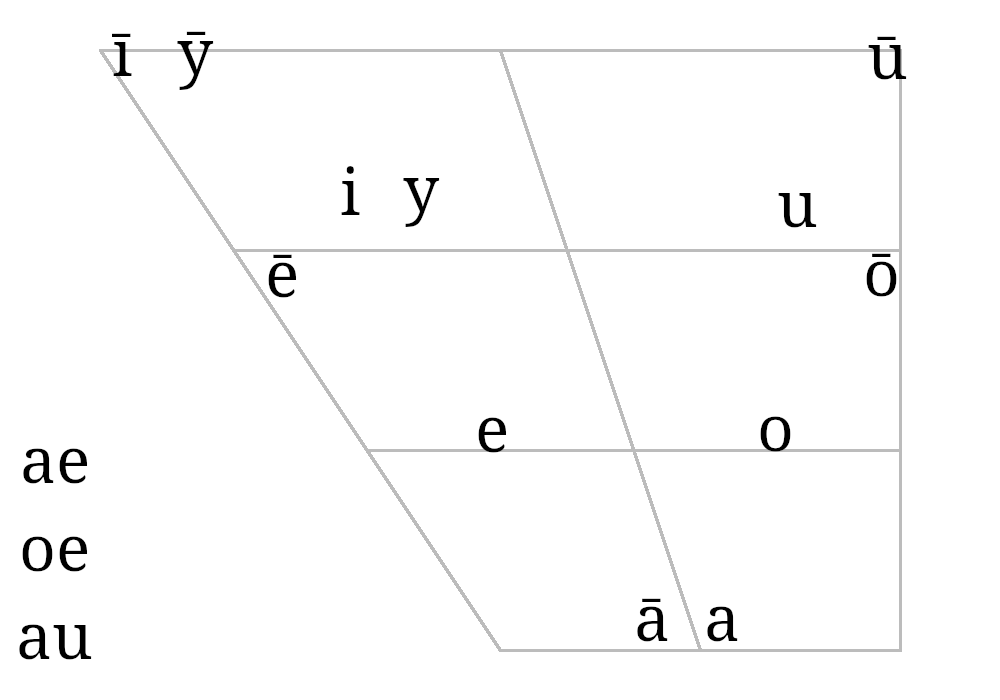
\includegraphics[width=\linewidth]{latin_vowels}
\end{frame}

\begin{frame}{Romance Vowels}
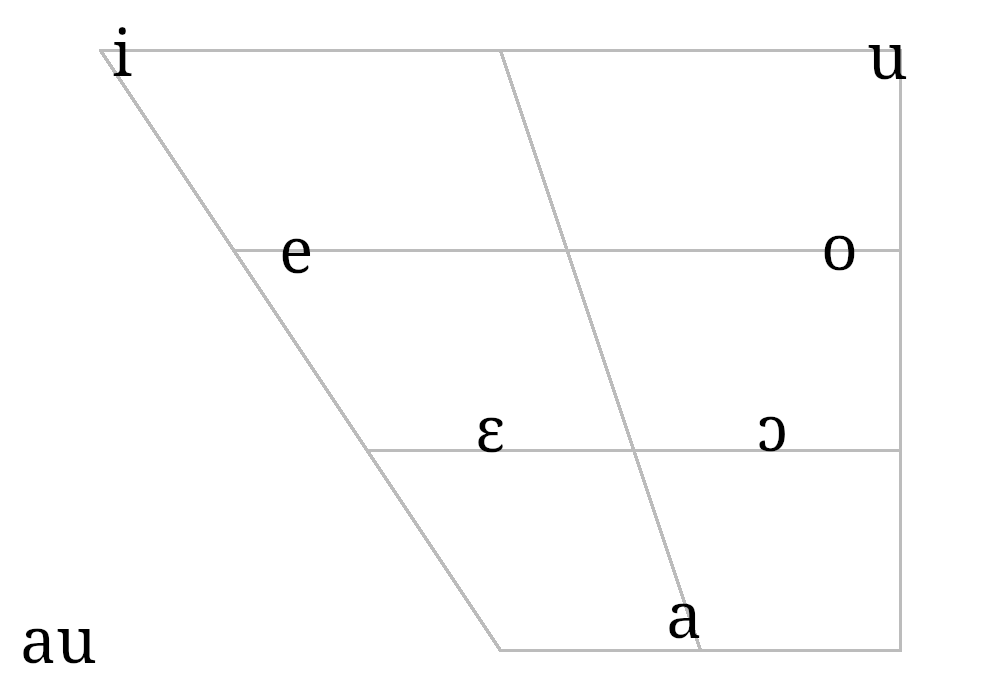
\includegraphics[width=\linewidth]{romance_vowels}
\end{frame}

\begin{frame}{Syllable Structure}
Cluster breaking:
\vspace{-1em}
\begin{itemize}
\item Latin \emph{spōnsa} ``fiancée'', Spanish \emph{esposa}
\item Latin \emph{strictus} ``tight'', Spanish \emph{estrecho}
\end{itemize}

Coda loss:
\vspace{-1em}
\begin{itemize}
\item Latin \emph{habētis} ``you (pl) have'', Italian \emph{avete}
\item Latin \emph{amābat} ``she was loving'', Spanish \emph{amaba}
\end{itemize}

Syncope:
\vspace{-1em}
\begin{itemize}
\item Latin \emph{viridis} ``green'', Italian, Spanish \emph{verde}
\item Latin \emph{calidum} ``hot'', Italian \emph{caldo}
\end{itemize}
\end{frame}

\begin{frame}{Syllable Structure}
Romance words are often shorter than their ancestors, due to syncope

But they're generally more \emph{restricted}: fewer phonemic vowels, fewer allowed clusters, fewer allowed onsets and codas

This reduces the informational load on each syllable, so the syllable rate can increase

The closest in speech rate is French: 14-17 vowels, many more codas (Italian \emph{caldo} but French \emph{chaud})
\end{frame}

\begin{frame}{Syllable Structure}
\includegraphics[width=\linewidth]{violin_global}
\end{frame}

\subsection{Future Directions}

\begin{frame}{What next?}
We believe these methods of extrapolation can be applied to other corpora

How much text is ``enough''? We can put bounds on this experimentally

Use Latin to test different measures of context

Interpolate between Latin and modern languages, see what impact different changes had

We've uncovered a phonetic property of a dead language that's been lost for two thousand years---and that's pretty cool
\end{frame}

\appendix

\section*{Appendix}
% Make a nice appendix marker slide
\begin{frame}{}
	\begin{centering}
	\begin{beamercolorbox}[sep=12pt,center]{section title}
	\usebeamerfont{section title}
	Appendix
	\end{beamercolorbox}
	\end{centering}
\end{frame}

\begin{frame}{With Digesta}
	\includegraphics[width=\linewidth]{jackknifing_yesdigesta}
\end{frame}

\begin{frame}{Without Cicero}
	\includegraphics[width=\linewidth]{jackknifing_nocicero}
\end{frame}

\subsection{Error}
\begin{frame}{Error calculation}
Multiple sources of uncertainty:
\vspace{-1em}
\begin{itemize}
\item Speech rate varies by person and occasion
\item The relationship between SR and ID isn't exact
\item Our ID is an estimate
\end{itemize}
\vspace{-1em}
We want to calculate a single distribution from this
\vspace*{-0.5em}
\begin{align*}
IR &= 39.15~\text{bit/sec} \quad & \quad \sigma_{IR} &= 5.10~\text{bit/sec} \\
ID &= 6.22~\text{bit/syl} \quad & \quad \sigma_{ID} &= 0.020~\text{bit/syl}
\end{align*}
\vspace*{-2em}
\begin{align*}
SR &= \frac{IR}{ID} = 6.29~\text{syl/sec} \\
\sigma_{SR} &= \sqrt{\left(\frac{\sigma_{IR}}{ID}\right)^2 + \left(\frac{\sigma_{ID}}{ID}\right)^2} = 0.82
\end{align*}
\end{frame}

\end{document}
